\chapter{Installation}

\section{Device setup}
%Turn off autosave

%Перейти в командный режим можно, установив USB Function в Control IO (см. п. 2.2. в высланном документе)

\section{Ubuntu linux}


\begin{verbatim}
cat /etc/udev/rules.d/60-yokogawa.rules 

SUBSYSTEM=="usb", ATTR{idVendor}=="0b21", ATTR{idProduct}=="0029", MODE="0666"
\end{verbatim}

logout and login

\section{Windows}

This section contains information on how to install the Software on Windows 10, but we hope that these steps work fine on Windows 7, Windows 11 or any future version.

\subsection{Checking prerequisites}

Python interpreter of version 3.10 or higher should be installed and added to the system path. We recommend to install the official Python distribution that can be downloaded from \url{https://www.python.org/downloads/}. The Python distribution from the Windows store doesn't work\footnote{The Python distribution from Windows store doesn't create \texttt{py.exe} file used to find the correct python version.}.

On Windows, you can check whether Python is installed by launching command prompt and typing
\begin{verbatim}
	C:/Users/UserName>py --version
	Python 3.10.5
\end{verbatim}
%\textbf{On Linux}, the version of Python interpreter can be checked by typing
%\begin{verbatim}
%	tea@tea-ubuntu>python3 --version
%	Python 3.10.5
%\end{verbatim}

For installation from sources, the computer should be connected to Internet to download the required libraries.

%We tested this software under Ubuntu 20.04 and 22.04, and Windows 10. We hope that this program will work fine under other versions of Linux and Windows due to the pythonic nature of it.


%The ``payload size'' of this software is about 20 MB, but it requires some third-party libraries to be installed. The overall size with these libraries is about 1 GB (the most huge library is PySide which is responsible for GUI). Therefore, we offer two types of installation: installation from the sources or installation from the self-contained zip archive.


\subsection{Driver installation}

The Software uses the \texttt{pyusb} library, which is a Python wrapper to the well known C library \texttt{libusb}. This library came from the world of Linux. Since Windows provides a different driver model to communicate with USB devices, the following additional step should be made.


The simplest way to install the correct driver is to use the Zadig software. This software is free and open source. It can be downloaded from 
\url{https://zadig.akeo.ie}
or using the direct link
\url{https://github.com/pbatard/libwdi/releases/download/v1.4.1/zadig-2.7.exe}.


To install generic winusdb driver, follow the instructions below (see Fig. \ref{fig:ZadigWnd}).
\begin{enumerate}
	\item Run \texttt{Zadig.exe} as Administrator
	\item Connect Yokogawa AQ7275 to a USB port of your computer. 
	\item Wait until Yokogawa AQ7275 appears in the drop box. Select this device in the drop box. If it didn't appear, try to uncheck and check again `Options/List all devices' from the main menu.
	\item Select the WinUSB driver. %This is a generic driver for usb devices.
	\item Press `Replace driver' or `Reinstall driver'.
\end{enumerate}

\begin{figure}[h!]
	\begin{center}
		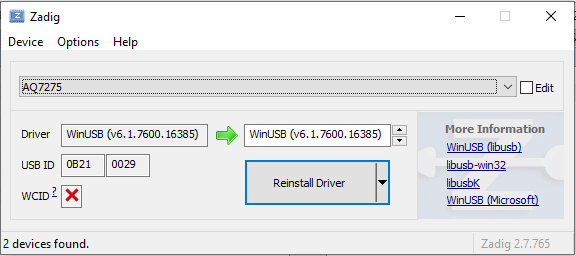
\includegraphics[width=12cm]{pictures/zadig.png}
	\end{center}
	\caption{Zadig window with selected WinUSB driver for Yokogawa AQ7275 device}
	\label{fig:ZadigWnd}
\end{figure}

The winusb driver should be installed only once. If Zadig software shows that winusb driver is already assigned to AQ7275, there is no need to install it again. 


\subsection{Installation}

\subsubsection{Unpacking}

First, we need to extract sources from the archive using any appropriate software. Let PATHTOSOURCES denote the path where the sources are placed, for example, \texttt{D:\textbackslash monitoring}. This path should contain the following files:
\dirtree{%
.1 monitoring.
.2 ...some subfolders.
.2 ...some other files.
.2 requirements.txt.
.2 install.bat.
.2 monitoringapp.py.
.2 monitoringapp.bat.
.2 libusb-1.0.dll (on Windows).
} 

\subsubsection{Automatic installation on Windows}
The simplest way to install the program is to execute \texttt{install.bat} by double-clicking or by typing the following commands in the command prompt:
\begin{verbatim}
cd <PATHTOSOURCES>
install.bat
\end{verbatim}

In case of problems, please, follow the commands in the next subsection to trace where the problems arises.

\subsubsection{Manual installation on Windows}\label{ss:manualInstallationOnWindows}

The \texttt{requirements.txt} file is sufficient to download and install all the dependencies that are not included in the sources. To do this, we need to create the virtual environment by typing the following commands:
\footnote{These commands create the virtual environment in the separate directory named \texttt{monitoring-env}. In general, the path to the virtual environment can be arbitrary, but the good choice is to place the virtual environment near the sources (or inside the sources).}

%\begin{verbatim}[On Linux]
%cd <PATHTOSOURCES>
%python3 -m venv monitoring-env
%source ./monitoring-env/bin/activate
%pip3 install -r requirements.txt
%\end{verbatim}

\begin{verbatim}
cd <PATHTOSOURCES>
py -m venv monitoring-env
monitoring-env\Scripts\activate.bat
pip3 install -r requirements.txt
\end{verbatim}

%Check, that PATHTOSOURCES folder contains file \texttt{libusb-1.0.dll}. This library is required by pyusb library to communicate via USB. 

\subsection{Running the program}
To run the program, just execute \texttt{monitoringapp.bat} by double-clicking. The second way to start the program is to type
%\begin{verbatim}[On Linux]
%cd <PATH-TO-SOURCES>
%source ./monitoring-env/bin/activate
%python3 -m monitoringapp
%\end{verbatim}

\begin{verbatim}
cd <PATH-TO-SOURCES>
set PATH=.;%PATH%
monitoring-env\Scripts\activate.bat
python3 -m monitoringapp
\end{verbatim}



%\subsubsection{Self-contained zipped distributive}


%To install the software, the following steps should be made. First, we need to create a separate virtual environment for this application:


